%##############################################################################
% Preamble
%##############################################################################
\documentclass[10pt,
               xcolor={usenames,dvipsnames},
               hyperref={colorlinks,linktoc=all,citecolor=Plum,linkcolor=MidnightBlue,urlcolor=MidnightBlue},noamssymb]{beamer}
% \usepackage[utf8]{inputenc}

% FONTS
\usepackage[T1]{fontenc}
\usepackage{tgtermes}
\usepackage{amsmath}

% Font choice 2:
\usepackage[scaled=0.92]{PTSans}
\usepackage{amssymb}
\newcommand{\mathbold}[1]{\ensuremath{\boldsymbol{\mathbf{#1}}}}
\newcommand{\mbf}[1]{\ensuremath{\boldsymbol{\mathbf{#1}}}}

% \usepackage{lmodern}

%\usefonttheme{professionalfonts}

\usepackage{scalefnt,letltxmacro}
\LetLtxMacro{\oldtextsc}{\textsc}
\renewcommand{\textsc}[1]{\oldtextsc{\fontfamily{lmr}\scalefont{1}#1}}

% \renewcommand*\ttdefault{lmvtt}
\usepackage[ttdefault=true]{AnonymousPro}

% GEOMETRY
%\usepackage[
%  paper  = letterpaper,
%  left   = 1.65in,
%  right  = 1.65in,
%  top    = 1.0in,
%  bottom = 1.0in,
%  ]{geometry}

% # COLOR

% \usepackage[usenames,dvipsnames]{xcolor}
\definecolor{shadecolor}{gray}{0.9}

% \newcommand{\red}[1]{\textcolor{BrickRed}{#1}}
% \newcommand{\orange}[1]{\textcolor{BurntOrange}{#1}}
% \newcommand{\green}[1]{\textcolor{OliveGreen}{#1}}
% \newcommand{\blue}[1]{\textcolor{MidnightBlue}{#1}}
% \newcommand{\sky}[1]{\textcolor{SkyBlue}{#1}}
% \newcommand{\gray}[1]{\textcolor{black!60}{#1}}

% SPACING and TEXT
%\usepackage[final,expansion=alltext]{microtype}
\usepackage[english]{babel}
\usepackage[parfill]{parskip}
\usepackage{afterpage}
\usepackage{framed}
\usepackage{xspace}

% LEFTBAR
\renewenvironment{leftbar}[1][\hsize]
{%
  \def\FrameCommand
  {%
    {\color{Gray}\vrule width 3pt}%
    \hspace{10pt}%
    %\hspace{0pt}\fboxsep=\FrameSep\colorbox{black!10}%
  }%
  \MakeFramed{\hsize#1\advance\hsize-\width\FrameRestore}%
}%
{\endMakeFramed}

% EDITING
% line numbering in left margin
\usepackage{lineno}
\renewcommand\linenumberfont{\normalfont
                             \footnotesize
                             \sffamily
                             \color{SkyBlue}}
% ragged paragraphs in right margin
\usepackage{ragged2e}
% TODO should i rename sidenote marginpar?
\DeclareRobustCommand{\sidenote}[1]{\marginpar{
                                    \RaggedRight
                                    \textcolor{Plum}{\textsf{#1}}}}
% paragraph counter in right margin
\newcommand{\parnum}{\bfseries\P\arabic{parcount}}
\newcounter{parcount}
\newcommand\p{%
    \stepcounter{parcount}%
    \leavevmode\marginpar[\hfill\parnum]{\parnum}%
}
% pargraph header
\DeclareRobustCommand{\parhead}[1]{\textbf{#1}~}
% paragraph helper
\DeclareRobustCommand{\PP}{\textcolor{Plum}{\P} }

% COUNTERS
%\renewcommand{\labelenumi}{\color{black!67}{\arabic{enumi}.}}
%\renewcommand{\labelenumii}{{\color{black!67}(\alph{enumii})}}
%\renewcommand{\labelitemi}{{\color{black!67}\textbullet}}

% FIGURES
\usepackage{graphicx}
\usepackage[labelfont=bf]{caption}
%\usepackage[format=hang]{subcaption}

% TABLES
\usepackage{booktabs}

% # ALGORITHMS

\usepackage[algoruled]{algorithm2e}
\setlength{\interspacetitleruled}{8pt}
\usepackage{listings}
\usepackage{fancyvrb}
\fvset{fontsize=\small}

% HYPERREF
%\usepackage[colorlinks,linktoc=all]{hyperref}
%\usepackage[all]{hypcap}
\hypersetup{citecolor=Plum}
\hypersetup{linkcolor=MidnightBlue}
\hypersetup{urlcolor=MidnightBlue}

% CLEVEREF must come after HYPERREF
\usepackage[nameinlink]{cleveref}
\newcommand{\Crefb}[1]{(\Cref{#1})}
\newcommand{\crefb}[1]{(\cref{#1})}

% ACRONYMS
\usepackage[acronym,smallcaps,nowarn]{glossaries}
\glsdisablehyper
% \makeglossaries

% COLOR DEFINITIONS
\newcommand{\red}[1]{\textcolor{BrickRed}{#1}}
\newcommand{\orange}[1]{\textcolor{BurntOrange}{#1}}
\newcommand{\green}[1]{\textcolor{OliveGreen}{#1}}
\newcommand{\blue}[1]{\textcolor{MidnightBlue}{#1}}
\newcommand{\gray}[1]{\textcolor{black!60}{#1}}

% CODE
\usepackage{minted}  % for syntax highlighting

% REFERENCES
\usepackage[
  backend=biber,
  natbib,
  doi=false,isbn=false,url=false,
  sorting=none,
  citestyle=authoryear]{biblatex}

\newacronym{PPL}{ppl}{probabilistic programming language}
\newacronym{GPU}{\textnormal{\uppercase{gpu}}}{graphics processing unit}

\newacronym{VAE}{vae}{variational auto-encoder}
\newacronym{RBM}{rbm}{restricted Boltzmann machine}
\newacronym{DLGM}{dlgm}{deep latent Gaussian model}
\newacronym{GAN}{gan}{generative adversarial network}
\newacronym{RNN}{rnn}{recurrent neural network}

\newacronym{VI}{vi}{variational inference}
\newacronym{MCMC}{mcmc}{Markov chain Monte Carlo}
\newacronym{MC}{mc}{Monte Carlo}
\newacronym{HMC}{hmc}{Hamiltonian Monte Carlo}
\newacronym{MAP}{map}{maximum a posteriori}
\newacronym{IWAE}{iwae}{importance-weighted auto-encoder}
\newacronym{HVM}{hvm}{hierarchical variational model}
\newacronym{KL}{kl}{Kullback-Leibler}
\newacronym{ELBO}{elbo}{\emph{evidence lower bound}}

\DeclareRobustCommand{\mb}[1]{\ensuremath{\boldsymbol{\mathbf{#1}}}}

\newcommand{\mba}{\mathbold{a}}
\newcommand{\mbb}{\mathbold{b}}
\newcommand{\mbc}{\mathbold{c}}
\newcommand{\mbd}{\mathbold{d}}
\newcommand{\mbe}{\mathbold{e}}
%\newcommand{\mbf}{\mathbold{f}}
\newcommand{\mbg}{\mathbold{g}}
\newcommand{\mbh}{\mathbold{h}}
\newcommand{\mbi}{\mathbold{i}}
\newcommand{\mbj}{\mathbold{j}}
\newcommand{\mbk}{\mathbold{k}}
\newcommand{\mbl}{\mathbold{l}}
\newcommand{\mbm}{\mathbold{m}}
\newcommand{\mbn}{\mathbold{n}}
\newcommand{\mbo}{\mathbold{o}}
\newcommand{\mbp}{\mathbold{p}}
\newcommand{\mbq}{\mathbold{q}}
\newcommand{\mbr}{\mathbold{r}}
\newcommand{\mbs}{\mathbold{s}}
\newcommand{\mbt}{\mathbold{t}}
\newcommand{\mbu}{\mathbold{u}}
\newcommand{\mbv}{\mathbold{v}}
\newcommand{\mbw}{\mathbold{w}}
\newcommand{\mbx}{\mathbold{x}}
\newcommand{\mby}{\mathbold{y}}
\newcommand{\mbz}{\mathbold{z}}

\newcommand{\mbA}{\mathbold{A}}
\newcommand{\mbB}{\mathbold{B}}
\newcommand{\mbC}{\mathbold{C}}
\newcommand{\mbD}{\mathbold{D}}
\newcommand{\mbE}{\mathbold{E}}
\newcommand{\mbF}{\mathbold{F}}
\newcommand{\mbG}{\mathbold{G}}
\newcommand{\mbH}{\mathbold{H}}
\newcommand{\mbI}{\mathbold{I}}
\newcommand{\mbJ}{\mathbold{J}}
\newcommand{\mbK}{\mathbold{K}}
\newcommand{\mbL}{\mathbold{L}}
\newcommand{\mbM}{\mathbold{M}}
\newcommand{\mbN}{\mathbold{N}}
\newcommand{\mbO}{\mathbold{O}}
\newcommand{\mbP}{\mathbold{P}}
\newcommand{\mbQ}{\mathbold{Q}}
\newcommand{\mbR}{\mathbold{R}}
\newcommand{\mbS}{\mathbold{S}}
\newcommand{\mbT}{\mathbold{T}}
\newcommand{\mbU}{\mathbold{U}}
\newcommand{\mbV}{\mathbold{V}}
\newcommand{\mbW}{\mathbold{W}}
\newcommand{\mbX}{\mathbold{X}}
\newcommand{\mbY}{\mathbold{Y}}
\newcommand{\mbZ}{\mathbold{Z}}

\newcommand{\mbalpha}{\mathbold{\alpha}}
\newcommand{\mbbeta}{\mathbold{\beta}}
\newcommand{\mbdelta}{\mathbold{\delta}}
\newcommand{\mbepsilon}{\mathbold{\epsilon}}
\newcommand{\mbchi}{\mathbold{\chi}}
\newcommand{\mbeta}{\mathbold{\eta}}
\newcommand{\mbgamma}{\mathbold{\gamma}}
\newcommand{\mbiota}{\mathbold{\iota}}
\newcommand{\mbkappa}{\mathbold{\kappa}}
\newcommand{\mblambda}{\mathbold{\lambda}}
\newcommand{\mbmu}{\mathbold{\mu}}
\newcommand{\mbnu}{\mathbold{\nu}}
\newcommand{\mbomega}{\mathbold{\omega}}
\newcommand{\mbphi}{\mathbold{\phi}}
\newcommand{\mbpi}{\mathbold{\pi}}
\newcommand{\mbpsi}{\mathbold{\psi}}
\newcommand{\mbrho}{\mathbold{\rho}}
\newcommand{\mbsigma}{\mathbold{\sigma}}
\newcommand{\mbtau}{\mathbold{\tau}}
\newcommand{\mbtheta}{\mathbold{\theta}}
\newcommand{\mbupsilon}{\mathbold{\upsilon}}
\newcommand{\mbvarepsilon}{\mathbold{\varepsilon}}
\newcommand{\mbvarphi}{\mathbold{\varphi}}
\newcommand{\mbvartheta}{\mathbold{\vartheta}}
\newcommand{\mbvarrho}{\mathbold{\varrho}}
\newcommand{\mbxi}{\mathbold{\xi}}
\newcommand{\mbzeta}{\mathbold{\zeta}}

\newcommand{\mbDelta}{\mathbold{\Delta}}
\newcommand{\mbGamma}{\mathbold{\Gamma}}
\newcommand{\mbLambda}{\mathbold{\Lambda}}
\newcommand{\mbOmega}{\mathbold{\Omega}}
\newcommand{\mbPhi}{\mathbold{\Phi}}
\newcommand{\mbPi}{\mathbold{\Pi}}
\newcommand{\mbPsi}{\mathbold{\Psi}}
\newcommand{\mbSigma}{\mathbold{\Sigma}}
\newcommand{\mbTheta}{\mathbold{\Theta}}
\newcommand{\mbUpsilon}{\mathbold{\Upsilon}}
\newcommand{\mbXi}{\mathbold{\Xi}}

\renewcommand{\d}[1]{\ensuremath{\operatorname{d}\!{#1}}}
\newcommand{\g}{\,|\,}
\renewcommand{\gg}{\,\|\,}
\newcommand\dif{\mathop{}\!\mathrm{d}}
\newcommand{\diag}{\textrm{diag}}
\newcommand{\supp}{\textrm{supp}}
\newcommand{\Gam}{\textrm{Gam}}
\newcommand{\InvGam}{\textrm{InvGam}}
\DeclareMathOperator*{\argmax}{arg\,max}
\DeclareMathOperator*{\argmin}{arg\,min}
\DeclareRobustCommand{\KL}[2]{\ensuremath{\textrm{KL}\left(#1\;\|\;#2\right)}}
\newcommand\indep{\protect\mathpalette{\protect\independenT}{\perp}}
\def\independenT#1#2{\mathrel{\rlap{$#1#2$}\mkern2mu{#1#2}}}
\newcommand{\E}[1]{\mathbb{E}\left[ #1 \right]}

\usepackage{tikz}
\usetikzlibrary{bayesnet}

\pgfdeclarelayer{edgelayer}
\pgfdeclarelayer{nodelayer}
\pgfsetlayers{edgelayer,nodelayer,main}

\definecolor{hexcolor0xbfbfbf}{rgb}{0.749,0.749,0.749}

\tikzset{>=latex}
\tikzstyle{none}   = [inner sep=0pt]
\tikzstyle{line}   = [-,
                      thick,
                      shorten <=1pt,
                      shorten >=1pt]
\tikzstyle{arrow}  = [->,
                      thick,
                      shorten <=1pt,
                      shorten >=1pt]
\tikzstyle{ardash} = [dashed,
                      ->,
                      thick,
                      shorten <=1pt,
                      shorten >=1pt]

\tikzstyle{empty}=[
                   circle,
                   opacity=0.0,
                   text opacity=1.0,
                   inner sep=0pt
                  ]

\tikzstyle{box}=[
                 rectangle,
                 fill=White,
                 thick,
                 draw=Black,
                 inner sep=7pt
                ]

\tikzstyle{filled}=[
                    circle,
                    thick,
                    fill=hexcolor0xbfbfbf,
                    draw=Black
                   ]

\tikzstyle{hollow}=[
                    circle,
                    thick,
                    fill=White,
                    draw=Black
                   ]

\tikzstyle{param}=[
                   rectangle,
                   fill=Black,
                   draw=Black,
                   inner sep=0pt,
                   minimum width=4pt,
                   minimum height=4pt
                  ]

\tikzstyle{paramhollow}=[
                         rectangle,
                         thick,
                         fill=White,
                         draw=Black,
                         inner sep=0pt,
                         minimum
                         width=4pt,
                         minimum height=4pt
                        ]

\usepackage{pgfplots}                               % PGFPLOTS baby!
\pgfplotsset{compat=newest}
\pgfplotsset{plot coordinates/math parser=false}
% \usepgfplotslibrary{statistics}


\usepackage{subfigure}
\definecolor{light}{RGB}{199, 153, 199}
\definecolor{dark}{RGB}{143, 39, 143}
\definecolor{gray80}{gray}{0.8}

\usepackage{natbib}
\setbeamertemplate{navigation symbols}{}
\setbeamertemplate{itemize items}[circle]
\setbeamercolor{itemize item}{fg=black!67}
\setbeamercolor*{enumerate item}{fg=black!67}
\setbeamercolor*{enumerate subitem}{fg=black!67}
\setbeamercolor*{enumerate subsubitem}{fg=black!67}

\definecolor{charcoal}{HTML}{222222}
\definecolor{snow}{HTML}{F9F9F9}

\setbeamercolor{background canvas}{bg=white}
\setbeamercolor{normal text}{fg=charcoal}
\setbeamercolor{structure}{fg=charcoal}

\newenvironment{changemargin}[1]{
  \begin{list}{}{
    \setlength{\topsep}{0pt}
    \setlength{\leftmargin}{#1}
    \setlength{\rightmargin}{#1}
    \setlength{\listparindent}{\parindent}
    \setlength{\itemindent}{\parindent}
    \setlength{\parsep}{\parskip}
  }
  \item[]}{\end{list}}

\title{}
\begin{document}

\begin{frame}[plain,t]
\begin{tikzpicture}[remember picture,overlay]
  \node [xshift=0.50cm, yshift=-3.00cm, anchor=north west] at (current page.north west) {
    \begin{tabular}{l}
    {\Large\bf Edward: A library for probabilistic modeling,}\\[1ex]
    {\Large\bf inference, and criticism}\\[2ex]
    {\large }\\[4ex]
    Dustin Tran, David M. Blei\\
    Columbia University\\[4ex]
    Matt Hoffman, Rif A. Saurous, Eugene Brevdo, \\
    Kevin Murphy \\
    Google Brain
    \end{tabular}
  };
  \node [xshift=-1.50cm, yshift=3.00cm, anchor=mid east] at (current page.south
  east) {
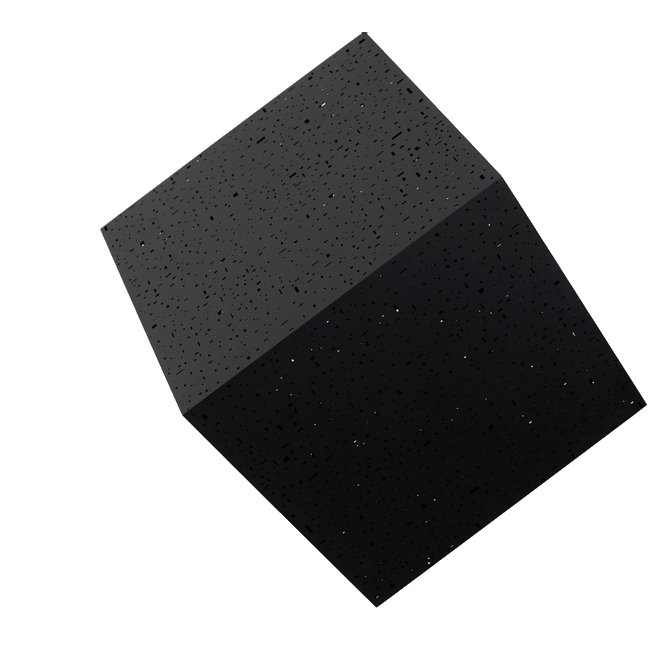
\includegraphics[width=0.25\textwidth]{img/edward.png}
  };
  \node [xshift=-1.30cm, yshift=2.45cm, anchor=mid east] at (current page.south
  east) {
\large \url{edwardlib.org}
  };
\end{tikzpicture}
\end{frame}

\begin{frame}
\frametitle{George E.P. Box (1919 - 2013)}
\begin{columns}
\begin{column}{0.5\textwidth}
    \begin{center}
     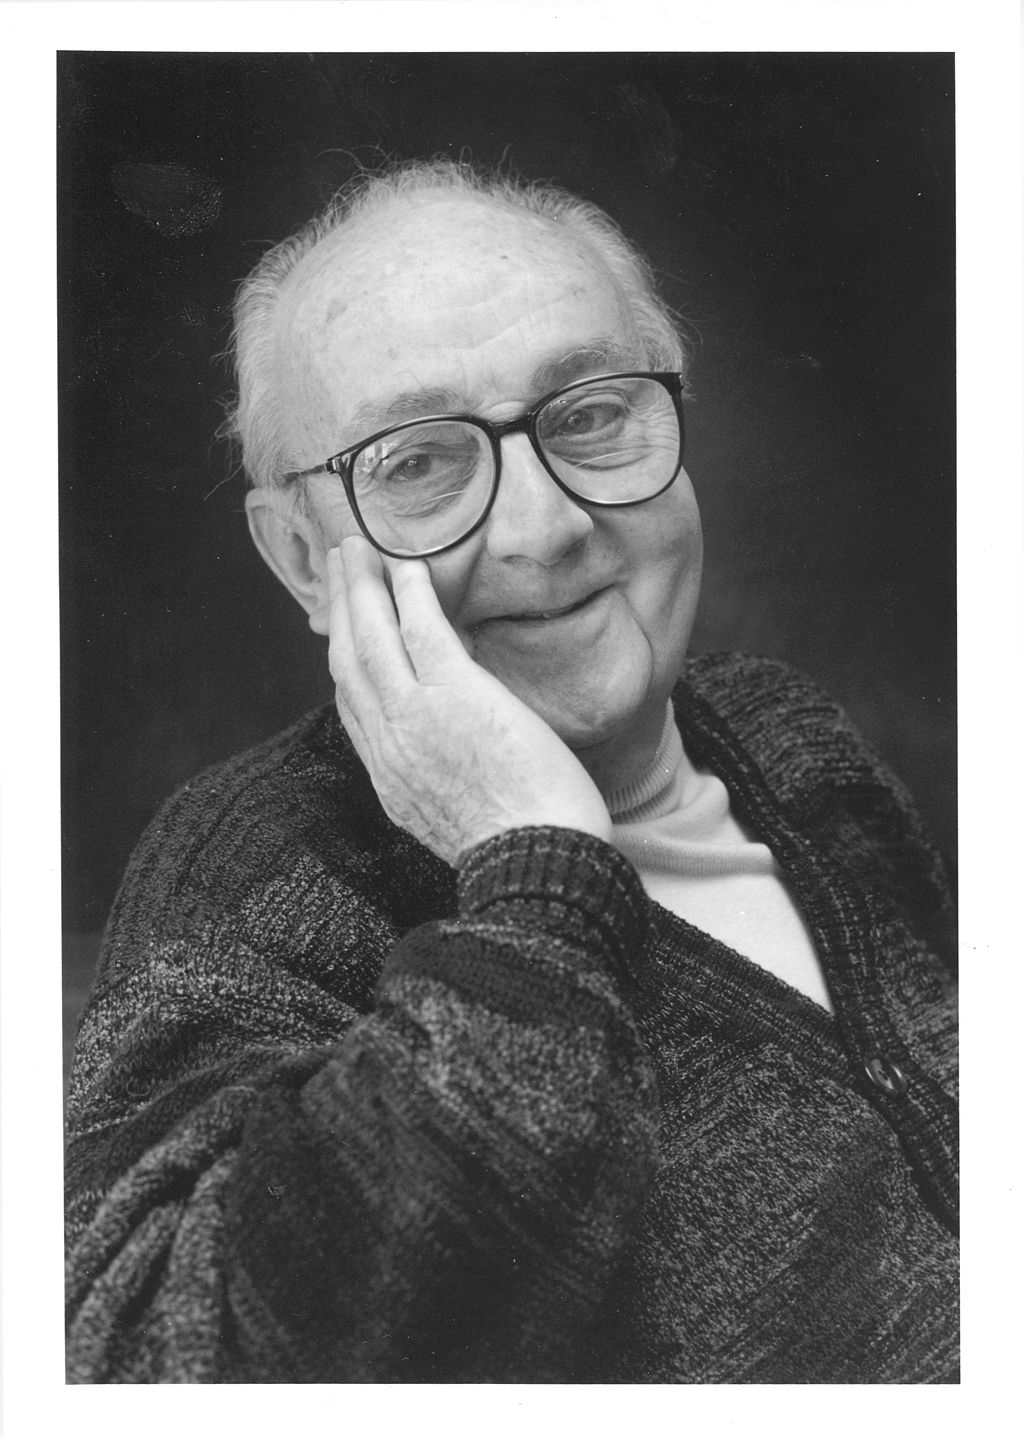
\includegraphics[width=\columnwidth]{img/box.jpg}
     \end{center}
\end{column}
\begin{column}{0.5\textwidth}
An iterative process for science:
\\[1ex]
\begin{enumerate}
\item Build a model of the science
\\[1ex]
\item Infer the model given data
\\[1ex]
\item Criticize the model given data
\end{enumerate}
\end{column}
\end{columns}
\begin{tikzpicture}[remember picture,overlay]
  \node [xshift=-9cm, yshift=0.4cm, anchor=south west] at (current
  page.south east) {
\gray{(Box \& Hunter 1962, 1965; Box \& Hill 1967; Box 1976, 1980)}
  };
\end{tikzpicture}
\end{frame}

\begin{frame}
\frametitle{Box's Loop}
\begin{tikzpicture}[remember picture,overlay]
  \node [xshift=-1cm, yshift=-2.00cm, anchor=north west] at (current page.north west) {
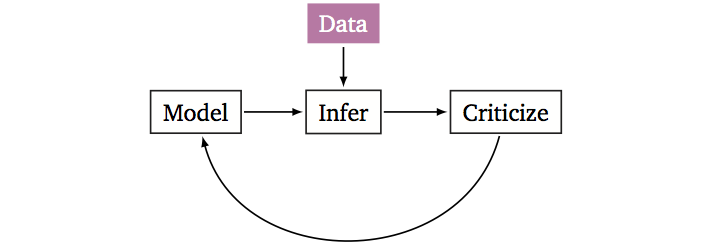
\includegraphics[width=1.4\textwidth]{img/model_infer_criticize.png}
  };
  \node [xshift=3.4cm, yshift=-8.0cm, anchor=north west] at (current page.north west) {
Edward is a library designed around this loop.
  };
  \node [xshift=0cm, yshift=-5.50cm, anchor=north west] at (current page.north west) {
  };
  \node [xshift=-5.0cm, yshift=0.4cm, anchor=south west] at (current
  page.south east) {
\gray{(Box, 1976; Box, 1980; Blei, 2014)}
  };
\end{tikzpicture}
\end{frame}

\begin{frame}
\vspace{3ex}
\textbf{Edward} is a probabilistic programming language,
designed for fast experimentation and research.

\emph{Modeling}
\begin{itemize}
\item
Composable Turing-complete language of random variables.
\item
Examples:
Graphical models, neural networks, probabilistic programs.
\item
Many data types, tensor vectorization, broadcasting, 3rd party support.
\end{itemize}

\emph{Inference}
\begin{itemize}
\item
Composable language for hybrids, message passing, data subsampling.
\item
Examples:
Black box VI, Hamiltonian MC, stochastic
gradient MCMC.
\item
Infrastructure to develop your own algorithms.
\end{itemize}

\emph{Criticism}
\begin{itemize}
\item
Examples: Scoring rules, hypothesis tests, predictive checks.
\end{itemize}

\vspace{1ex}
Built on TensorFlow (features distributed computing, GPUs, autodiff).

\begin{tikzpicture}[remember picture,overlay]
  \node [xshift=-3cm, yshift=0.4cm, anchor=south west] at (current
  page.south east) {
\gray{(Tran et al., 2016)}
  };
\end{tikzpicture}
\end{frame}

\begin{frame}
\begin{center}
\vspace{-4ex}
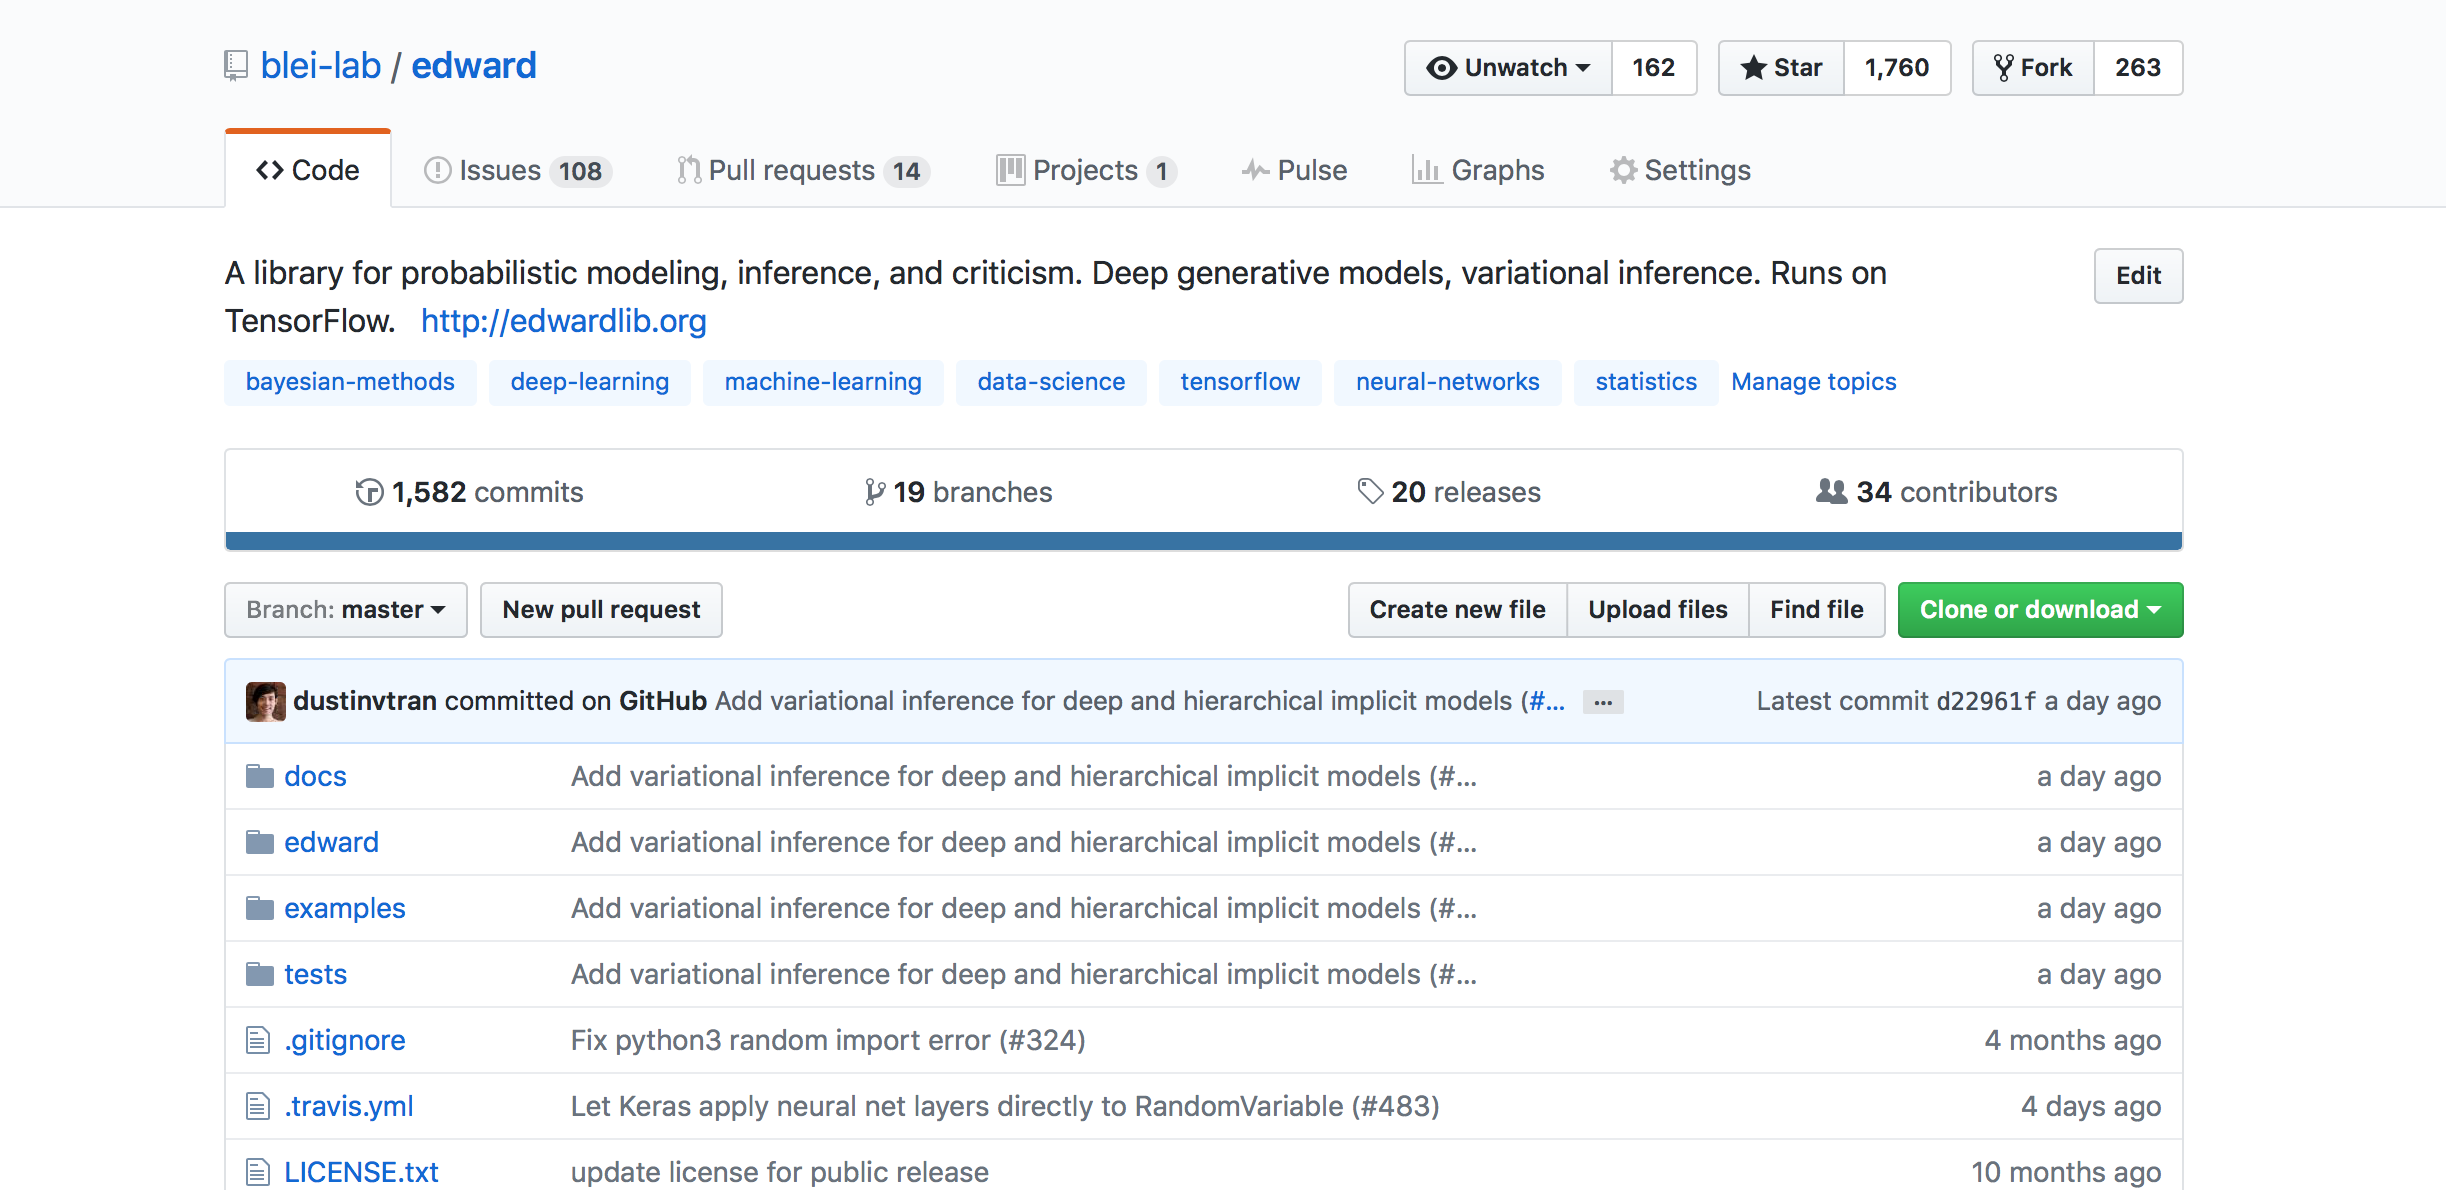
\includegraphics[width=1.1\textwidth]{img/github.png}
\\

\includegraphics[width=1.0\textwidth]{img/gitter.png}
\\[3ex]
\end{center}
We have an active community of several hundred users. We have
many few-commit developers.
\end{frame}

\begin{frame}
\frametitle{Who is Using Edward?}
{\large Users}
\begin{enumerate}
\item
Machine learning enthusiasts, data scientists, business analysts \\
(\emph{ex. hierarchical GLMs, mixture models, MAP, MCMC, ...})
\item
Probabilistic graphical modeling community \\
(\emph{ex. latent Dirichlet allocation, variational inference, Gibbs})
\item
Bayesian deep learning community \\
(\emph{ex. deep generative models, Bayesian NNs, black box inference})
\end{enumerate}

{\large Developers}
\begin{enumerate}
\item
David Blei's group
\item
Google Brain
(\emph{in conception/design})
\item
Matt Hoffman (\emph{conjugacy}),
Emily Fox's group
(\emph{time series + SGMCMC}),
Justin Bayer (\emph{stochastic RNNs}),
John Pearson (\emph{neuroscience}),
a few Master's/Ph.D. students.
\item
Everyone is part-time. Collaboration continues to evolve.
\end{enumerate}
\end{frame}

\begin{frame}[plain,t]
\frametitle{Variational Auto-Encoder}
\begin{tikzpicture}[remember picture,overlay]
  \node [xshift=12.40cm, yshift=3.5cm, anchor=mid east] at (current page.south
  west) {
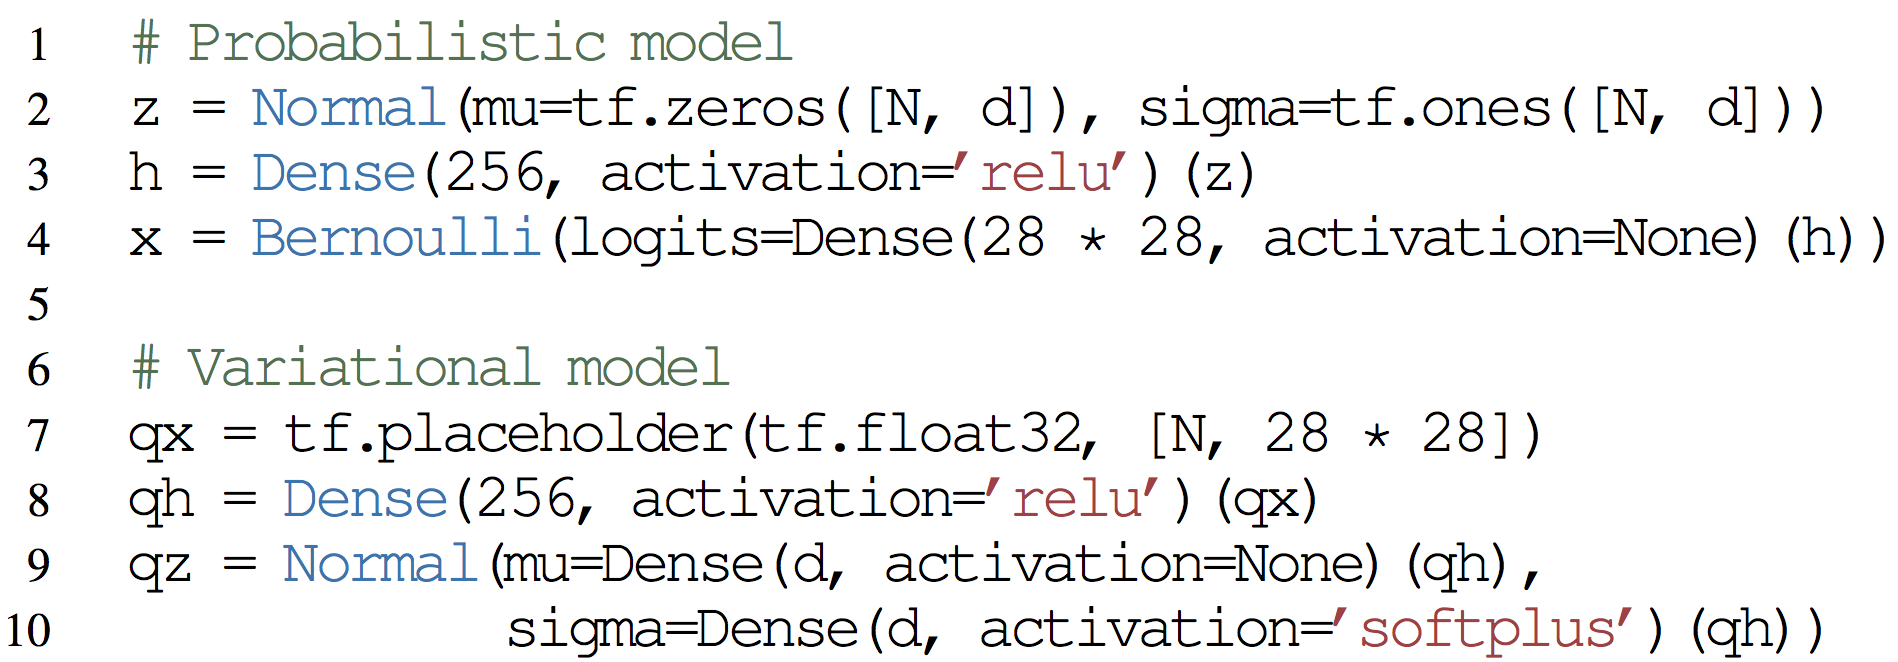
\includegraphics[width=0.9\textwidth]{img/vae_code.png}
  };
  \node [xshift=3.00cm, yshift=3.25cm, anchor=mid east] at (current page.south
  west) {
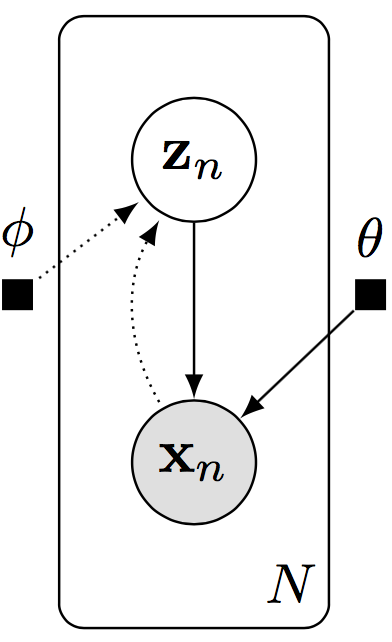
\includegraphics[width=0.20\textwidth]{img/vae_graph.png}
  };
\end{tikzpicture}
\end{frame}

\begin{frame}[plain,t]
\frametitle{Generative Adversarial Network}
\begin{tikzpicture}[remember picture,overlay]
  \node [xshift=12.50cm, yshift=2.8cm, anchor=mid east] at (current page.south
  west) {
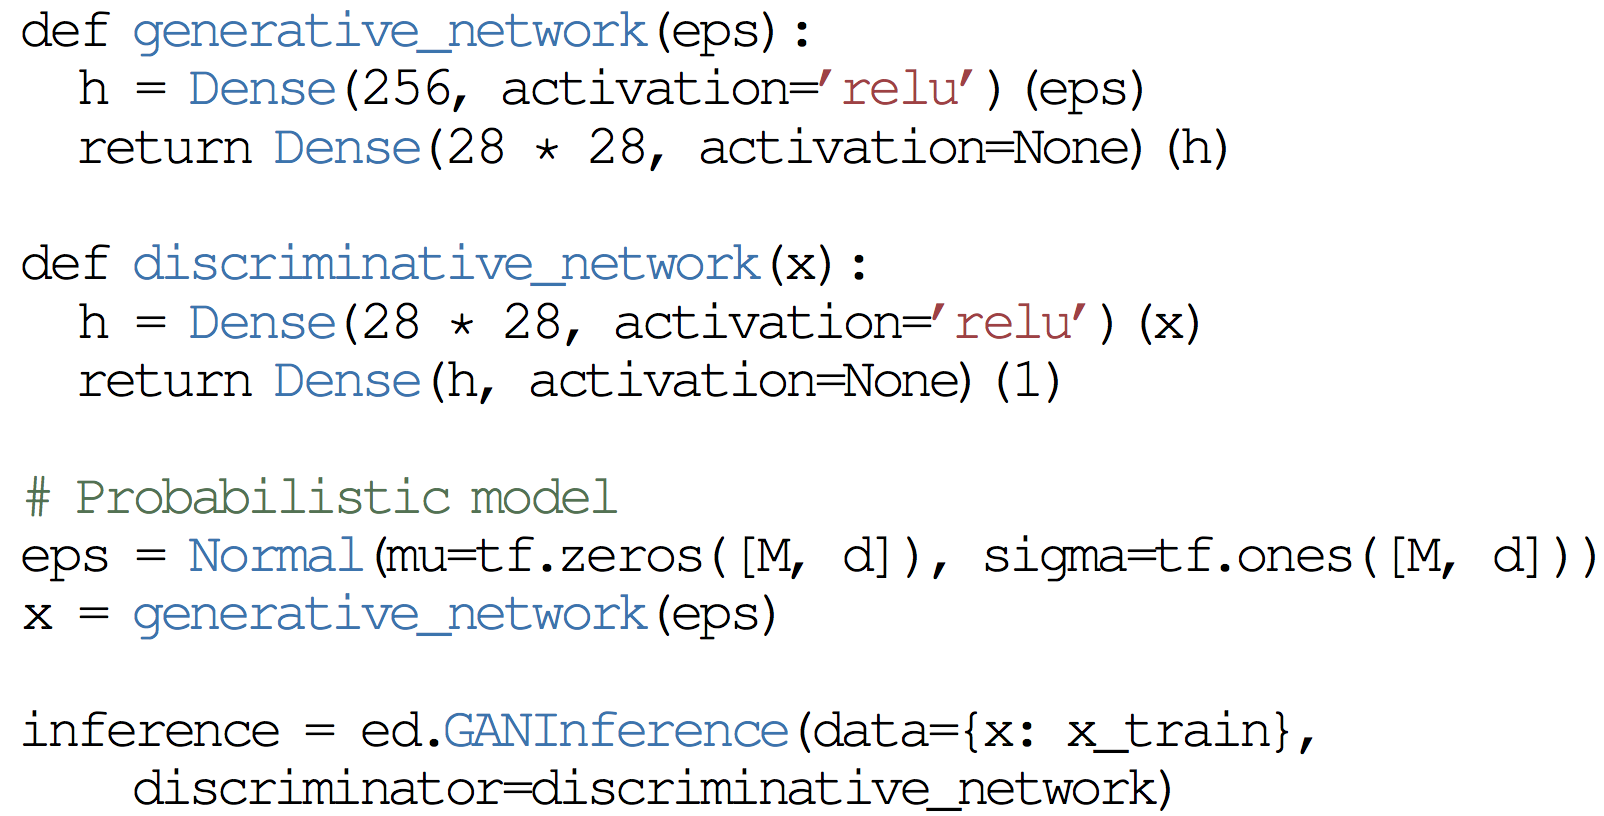
\includegraphics[width=0.85\textwidth]{img/gan_code.png}
  };
  \node [xshift=3.20cm, yshift=3.25cm, anchor=mid east] at (current page.south
  west) {
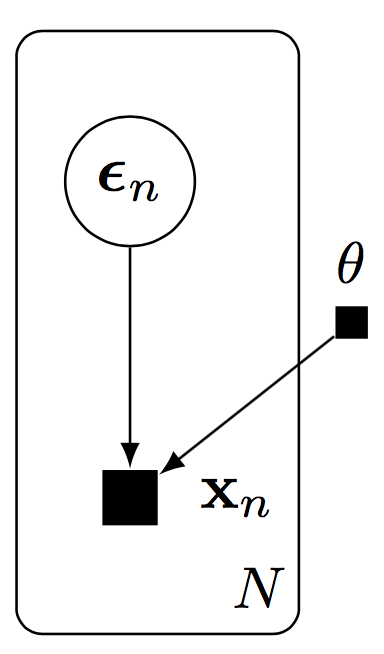
\includegraphics[width=0.20\textwidth]{img/gan_graph.png}
  };
\end{tikzpicture}
\end{frame}

\end{document}
